\documentclass[a4paper]{article}
% *** Packages
\usepackage[left=2cm,right=2cm,top=2cm,bottom=2cm]{geometry}
\usepackage{graphicx}
\usepackage{tabularx}
\usepackage{isomath}
\usepackage{mathrsfs}
\usepackage{subfigure}	
\usepackage{fancyhdr}
\usepackage{epstopdf}
\usepackage{bm}
\usepackage{color}
\usepackage{xcolor}
\usepackage{listings}
\usepackage[T1]{fontenc}
\usepackage{amssymb,amsmath}
\usepackage{multirow}
\usepackage{tablefootnote}
\usepackage{threeparttable}
\usepackage{array}
\usepackage{cite}
\usepackage{comment}
\usepackage{url}
\usepackage{hyperref}

\setlength{\parindent}{0pt}
\parskip 5mm
\renewcommand{\baselinestretch}{1.1}

\title{A \textit{Git} Tutorial}
\author{sunlu.electric@gmail.com}
\date{\today}

\begin{document}
\maketitle

\textit{Git} is a distributed version-control system for tracking changes in source code during software development, and it can be used in cross platforms including Windows OS, Unix/Linux and MacOS. This tutorial introduces the basic use of \textit{Git} on a local Linux machine and on a remote host such as \textit{GitHub}.

\tableofcontents

\section{Introduction to \textit{Git} and \textit{GitHub}}

\textit{Git}, created by Linus Trovalds in 2005, is a distributed version-control system for tracking changes in source code and files during software development. It is designed for coordinating work among programmers and its goals include speed, data integrity and support for distributed non-linear work flows. \textit{Git} is a free and open-source piese of software under GNU general public license V2.

As with most other distributed version-control systems, every \textit{Git} directory on every local computer is a full-fledged repository with complete history and full version-tracking abilities, independent of network access or a central server \cite{wikipediaGit}. A demonstration of how \textit{Git} utilizes master and slave repositories (also known as ``branches'') to coordinate projects is given in Fig. \ref{fig:Gitrepositorydemo}. A ``master repository'' is used as a shared repository where everyone pull the updated version of the project, make modifications, then push back the modified project. Each branch, when pulled, is a duplication of the master repository thus contains the entire project files.

\begin{figure}[htbp]
    \centering
    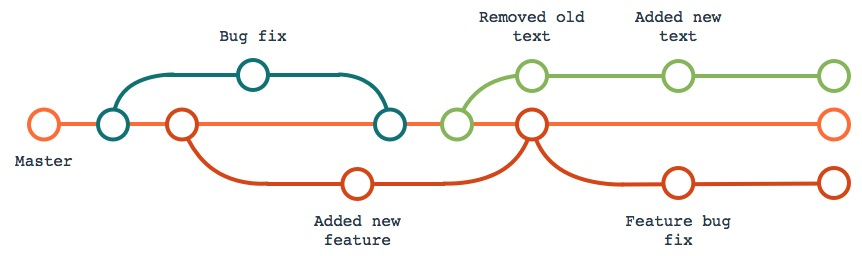
\includegraphics[width=0.8\textwidth]{figGitrepositorydemo.jpg}
    \caption{A demonstration of how \textit{Git} repositories work to coordinate programmers code \cite{blogGitVersionControl}. }
    \label{fig:Gitrepositorydemo}
\end{figure}

\textit{GitHub} is a global company that provides hosting for software development version control using \textit{Git}. It offers all of the distributed version control and source code management functionality of \textit{Git} and also adds its own features. It provides access control and several collaboration features such as bug racking, task management and wikis for each project \cite{wikipediaGitHub}. \textit{GitHub} offers plans for free, professional and enterprise accounts. It offers unlimited private repositories to all the plans, and has become the largest host of source code in the world as of May 2019.

Notice that \textit{GitHub} is not the only company that provides this kind of services. Other companies, for example \textit{GitLab}, also provide similar services.

\section{\textit{Git} on a Local Linux Machine}

\subsection{Install \textit{Git}}

\textit{Git} is a build-in software in most (if not all) Linux distributions. The following commands in shell should download and install \textit{Git} on a Linux machine.
\begin{lstlisting}[backgroundcolor = \color{lightgray},language=bash]
  $ sudo apt install git
\end{lstlisting}

The user name and email can be configured as follows. Notice that this configuration is global to all \textit{Git} projects in the machine.
\begin{lstlisting}[backgroundcolor = \color{lightgray},language=bash]
  $ git config --global user.name 'user_name'
  $ git config --global user.email 'user_email@user_domain'
\end{lstlisting}

\subsection{Create a \textit{Git} Project and Add/Remove Files}

Consider creating a \textit{Git} project and work on it on a local machine. As a first step, create an empty folder for the project. Navigate to the project folder. Use the following bash command to initialize a \textit{Git} project repository.
\begin{lstlisting}[backgroundcolor = \color{lightgray},language=bash]
  $ git init
\end{lstlisting}
By doing this, the project is initialized and further \textit{Git} commands can be applied to it. Behind the screen, a hidden folder \texttt{.git} has been automatically created in the project folder, containing the metadata of the project. It is not necessary to manually access this hidden folder.

In each step of the project development, always use the following command to check the \textit{Git} status, including the project files status information and versions information.
\begin{lstlisting}[backgroundcolor = \color{lightgray},language=bash]
  $ git status
\end{lstlisting}

With the current directory initialized by \colorbox{lightgray}{git status}, the following commands add a file that already exists in the directory to \textit{Git}.
\begin{lstlisting}[backgroundcolor = \color{lightgray},language=bash]
  $ git add <file_name>
\end{lstlisting}

The process of adding a file to \textit{Git} is considered as a change, thus leaving these files in the staging area, whose concept is illustrated by Fig. \ref{fig:StagingArea}. The file needs to be committed later on before the change is actually confirmed. For a file that is in the project folder but not added to \textit{Git}, it is considered as untracked file. Use \colorbox{lightgray}{git status} to check the status of all files in the project folder.
\begin{figure}[htbp]
    \centering
    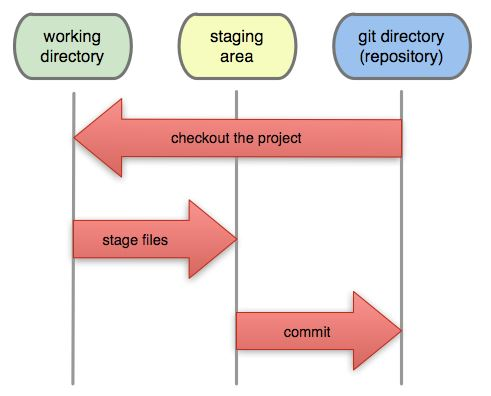
\includegraphics[width=0.5\textwidth]{figStagingArea.jpg}
    \caption{A demonstration of how staging area works \cite{stackexchangeStagingArea}. }
    \label{fig:StagingArea}
\end{figure}

To remove a file from \textit{Git}, use the following commands. The removed file will then appear in the untracked file list.
\begin{lstlisting}[backgroundcolor = \color{lightgray},language=bash]
  $ git rm --cached <file_name>
\end{lstlisting}

Regular expression can be used in the above commands.

\subsection{Commit a Project File in the Staging Area}

The existing files in \textit{Git} can be modified with any file editor. When changes are made to such files, they will be automatically put into the staging area (just like when a new file is added to \textit{Git}).

Using the following command to commit all files in the staging area. A \textit{vim} editor will pop up and ask the user to put in comments to the commit. The comments are mandatory.
\begin{lstlisting}[backgroundcolor = \color{lightgray},language=bash]
  $ git commit
\end{lstlisting}

When committing the files, the name and email information of the author and committer will be recorded. The information is taken from environment variables if set the following 6 variables.
\begin{itemize}
  \item GIT\_AUTHOR\_NAME
  \item GIT\_AUTHOR\_EMAIL
  \item GIT\_AUTHOR\_DATE
  \item GIT\_COMMITTER\_NAME
  \item GIT\_COMMITTER\_EMAIL
  \item GIT\_COMMITTER\_DATE
\end{itemize}
If they are not set, the information is taken from \textbf{user.name} and \textbf{user.email}, or \textbf{/etc/mailname}, or \textbf{\$HOSTNAME} of the machine.

There are some commonly used options for the commit command.
\begin{lstlisting}[backgroundcolor = \color{lightgray},language=bash]
  $ git commit [-a]                 # Commit all files
               [<file_name>]        # Commit a particular file
               [--author=<author>]  # Override the commit author
               [-m <message>]       # One line comment, instead of vim comment
\end{lstlisting}

File \textit{.gitignore} in the directory can be used as a ignore list for \textit{Git}. Files and directories that are added into \textit{.gitignore} will not be monitored or tracked by \textit{Git}. However, do notice that \textit{.gitignore} will be monitored and tracked by \textit{Git}. Regular expressions can be used in \textit{.gitignore} file as well. This becomes handy when there is a log file in the directory which does not necessarily need to be tracked.

\subsection{Work on Different Branches}

By default, when a project is created, the user works on the Master branch. This is reflected when using \colorbox{lightgray}{git status}, where it is shown \textit{``On branch Master''}. Therefore, all the commit mentioned in the previous section is done on Master branch.

In practice, it is more often that a separate branch is created for a particular upgrade or modification purpose. Only when the functions in the separate branch has been tested, would it be merged to the master branch. This is shown in Fig. \ref{fig:Gitrepositorydemo}.

Using the following command to create a branch. Notice that this does not change the current branch automatically.
\begin{lstlisting}[backgroundcolor = \color{lightgray},language=bash]
  $ git branch <branch_name>
\end{lstlisting}

Use the following command to switch branch.
\begin{lstlisting}[backgroundcolor = \color{lightgray},language=bash]
  $ git checkout <branch_name>
\end{lstlisting}

At this moment, all commit made using \colorbox{lightgray}{git commit} will be done on the switched new branch. All the changes made on this branch, including the changes in the staging area and yet not committed, are transparent to other branches including the Master branch.

The new branch can be merged to the master as follows. First, switch back to master branch. Then, use the following command. A \textit{vim} editor will pop up and ask the user to put in comments to the commit. The comments are mandatory.
\begin{lstlisting}[backgroundcolor = \color{lightgray},language=bash]
  $ git merge <branch_name>
\end{lstlisting}

This create-switch-merge branches approach is handy for version control especially in collaborative projects.

\section{\textit{Git} on Remote Repository (Such as \textit{GitHub})}

\subsection{Register a Remote Repository}

To use \textit{GitHub}, the user needs to register a \textit{GitHub} account and create a repository. Then the \textit{GitHub} repository can be added to the local machine as a remote repository as follows.
\begin{lstlisting}[backgroundcolor = \color{lightgray},language=bash]
  $ git remote add <remote_name> <remote_url> # Add remote repository
  $ git remote rename <old_remote_name> <remote_name> # Change remote_name
  $ git remote set-rul <remote_name> <new_remote_url> # Change remote_url
  $ git remote remove <remote_name> # Remove remote repository
\end{lstlisting}
For example,
\begin{lstlisting}[backgroundcolor = \color{lightgray},language=bash]
  $ git remote add raspi4b https://github.com/sunluelectric/raspi4b.git
\end{lstlisting}

Notice that the remote name is not necessarily the same with the repository name in \textit{GitHub}. It is simply the name by which the local \textit{Git} is tracking the access point. Use \colorbox{lightgray}{git remote -v} to check all remote access points stored in the local machine.

Authentication is required when the user interact with the remote repository from the local machine.

The use of the above method to register a remote repository is not limited to \textit{GitHub}. The same method can be applied to other remote \textit{Git} management system.

\subsection{Download a Clone of a Project}

Use \colorbox{lightgray}{git clone} to download an existing repository from remote repository as follows. A new directory is created on the local machine for this repository.
\begin{lstlisting}[backgroundcolor = \color{lightgray},language=bash]
  $ git clone <repository_url> [<directory>]
\end{lstlisting}

When using \colorbox{lightgray}{git clone}, the repository is automatically added into \colorbox{lightgray}{git remote}, and all branches change on the remote repository are tracked. If changes, for example updated, are made to the remote repository, \colorbox{lightgray}{git pull} can be used to pull the changes.

\subsection{Pull Updates and Push Changes from/to Remote Repository}

Use \colorbox{lightgray}{git pull} to download the latest version of a branch in the repository. It is configurable what to be carried out when the existing local versions conflicts with the existing remote versions.
\begin{lstlisting}[backgroundcolor = \color{lightgray},language=bash]
  $ git pull [<options>] [<repository>]
\end{lstlisting}

Use \colorbox{lightgray}{git push} to upload a file, or more often, a branch, into the remote repository. Usually, the changes made in the local machine has already been committed to a branch and \colorbox{lightgray}{git push} will upload the updated branch to the remote repository.
\begin{lstlisting}[backgroundcolor = \color{lightgray},language=bash]
  $ git push [<options>] [--repo=<repository>]
\end{lstlisting}
The authentication is required when pushing changes to the remote repository.

\bibliographystyle{IEEEtran}
\bibliography{references}

\end{document} 